\documentclass[12pt]{article}                                                                                                                       
\usepackage{sbc-template}                                                 
\usepackage{graphicx,url}                                                 
\usepackage[utf8]{inputenc}                                               
\usepackage[brazil]{babel}                                                      
\usepackage{graphicx}

\title{Assignment 2 \\ Teoria de Grafos e Computabilidade}
\author{Iyan Lucas Duarte Marques\inst{1}, Samir do Amorim Cambraia\inst{1}}

\address{Instituto de Ciências Exatas e Informática - Pontifícea Universidade Católica Minas Gerais (PUC-MG)}

\begin{document}

\maketitle

\section{Problema}
\textit{"
	O problema de se determinar o número máximo de caminhos disjuntos em arestas existentes em um grafo
	apresenta várias aplicações. Neste trabalho você deverá implementar um método de resolução deste problema que receba
	um grafo e um par de vértices (isto é, origem e destino) exiba ao final a quantidade de caminhos disjuntos em arestas
	entre os dois vértices dados, além de listar cada um dos caminhos encontrados.
	"}
    \begin{center}
        \begin{figure}[h!]
            \centering
            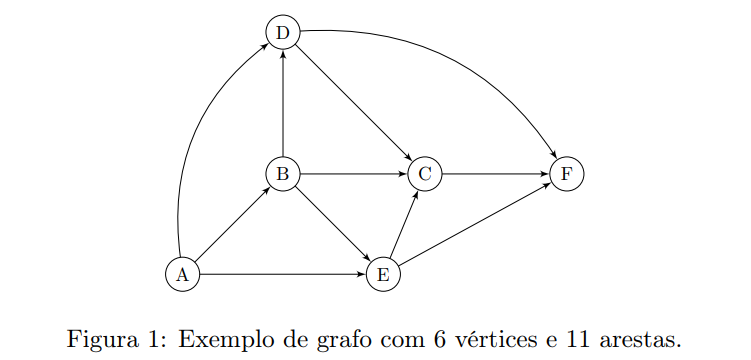
\includegraphics[width=1\textwidth]{imagens/figura-1.png}
        \end{figure}
    \end{center}

\section{Implementação}
\subsection{A classe}
\subsubsection{Construtor}
O objeto recebe um object, que é na verdade um dicionário de dicionários, onde cada vértice é um dicionário. 
A chave do dict por sua vez é o rótulo do vértice e os values são os outros vértices onde há uma aresta que incide nos mesmos.
Desta forma, se o object está vazio, é gerado um dicionário vazio como variável local da classe para substituí-lo.

\subsubsection{Vertices e Arestas}
Quando nós adicionamos um object na construção do objeto de classe, ele atribui automaticamente os vertices e arestas.
Entretanto, quando quisermos adicionar um vértice, o código simplesmente adiciona-o no dicionário de vértices.
Já com as arestas, é um pouco mais complicado, o código recebe as arestas, sendo as arestas um parâmetro, e atribui como um valor no dicionário do vértice $X$.
O valor é uma tupla, onde é o $($incidente, origem$)$ e guardado no object.

\subsubsection{\textit{Path}}
Para achar um caminho, há o vertice inicial e o destino. 
Se o caminho existe e o vértice inicial não é o final, a função viaja recursivamente por cada vértice que há uma ligação.
Ou seja, a função é chamada internamente passando pelo parâmetro o vértice atual, e o vértice de destino original e o array de caminho (que é anexado a cada iteração).
Para achar todos os caminhos é literalmente a forma que se roda mais vezes só que o array de caminho diferente (isso possibilita a ele escolher caminhos que não foram selecionados) e então anexados em um array de caminhos.


\section{Utilização}
\subsection{Execução}
Para executar o código, precisa-se estar no diretório  e digitar o comando \textit{python main.py}.

\subsection{Arquivos}
\begin{itemize}
	\item \textbf{\textit{main.py:}}
	      Arquivo que contem a declaração do grafo e a chamada dos métodos.
	\item \textbf{\textit{grafo.py:}}
	      Arquivo que contem a classe grafo declarada e com seus métodos.
\end{itemize}


\end{document}